\chapter{Introduction}
\label{cha:introduction}

\section{Macroscopic City Movements - problem definition}
\label{cha:introduction_probdef}

\textbf{Here we should describe what problem project is about to solve. In the 1st term presentation I mentioned that we want to answer two questions:
}\\
 
Given a location, where and in what proportion people move to another location - Movement Graph? 
\\
Where and how long do people stay at certain location? - but we need to be more precise here.

\FloatBarrier

\section{Human Mobility within the city}
\label{cha:introduction_hummob}

According to research \cite{HumanMobility1}\cite{HumanMobility2}\cite{HumanMobility3}, the average walking speed in the city for man aged 40 is 1.4 m/s (5 km/h), and slowest one is for elderly (with walking impairment) below 1 m/s (3.6 km/h). 

\FloatBarrier

\section{Methodology of obtaining location data}
\label{cha:introduction_methodo}

Here we should describe how and from where do we get the data, and emphasise the fact that location updates are based on MOVEMENTS, so each next point is triggered by some mobile phone movement. Point updates are not triggered while being stationary.
\\
TODO: we need here more details about what our Sudanian guy were supposed to research
\begin{figure}[!ht]
	\centering
	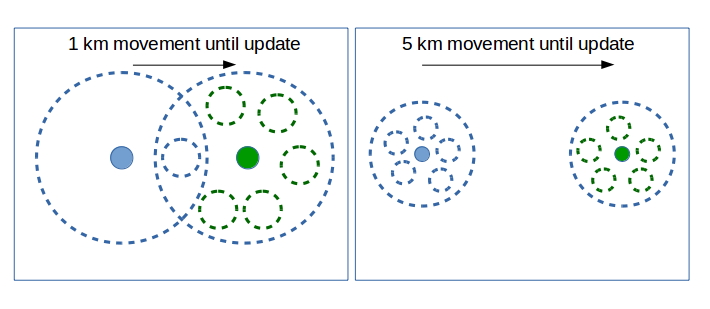
\includegraphics[width=0.9\textwidth]{images/movement_update.png}\\
	\caption{Continuous and Discontinuous location update after movement to section lacking area details  }
	\label{fig:introduction_movement_update}
\end{figure}
\FloatBarrier

\section{Location data characteristics for Berlin area}

\subsection{General overview}

Movement triggered data from mobile devices are spanned across the Germany as shown on \autoref{fig:introduction_ger_points}. 
\\
\begin{figure}[!ht]
	\centering
	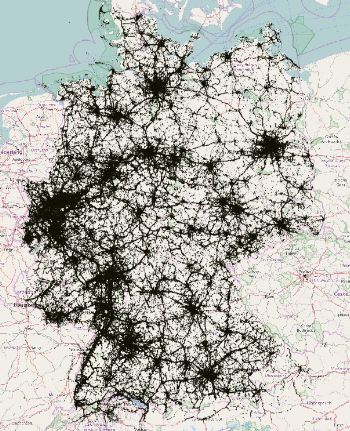
\includegraphics[width=0.3\textwidth]{images/points_germany.png}\\
	\caption{Visualisation of data points location in the geographical map of Germany}
	\label{fig:introduction_ger_points}
\end{figure}
\\
It points out, that most of the detected movements from one point to another are mostly gathered on the highways and inside the cities. 
\\
\begin{figure}[!ht]
	\centering
	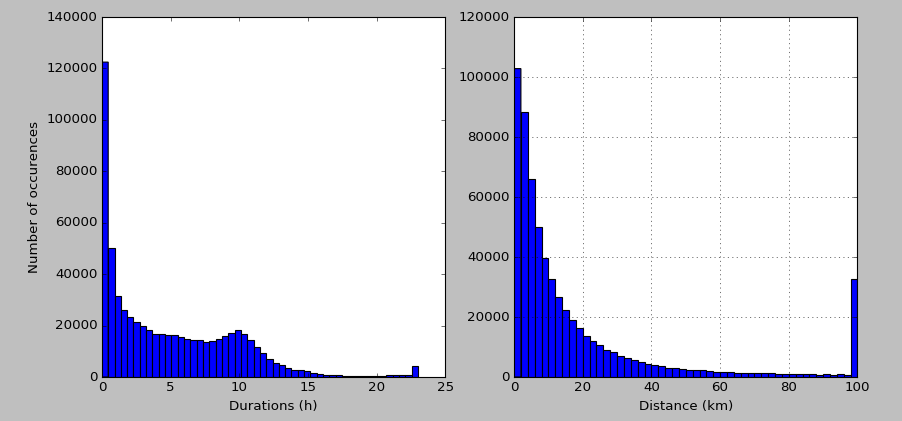
\includegraphics[width=0.9\textwidth]{images/germany_stats.png}\\
	\caption{Histograms of durations and distances between consecutive points under and cumulatively over 100 km for the area of Germany}
	\label{fig:introduction_ger_stats}
\end{figure}
\\
The given data batch has been gathered in the interval of 24h starting from 3am in the morning German time. It consists of over 675000 data points, belonging to 47300 unique mobile devices. \autoref{fig:introduction_ger_stats} shows, that for unique mobile devices, the durations between consecutive points in time are most frequent within 30 minutes and most of the data is in the interval 1-10h. Regarding distances, consecutive points are most frequent below 2 km and most data is in the interval 0-10km. Big chunk of distances is also over 100km.     
\\
\begin{figure}[!ht]
	\centering
	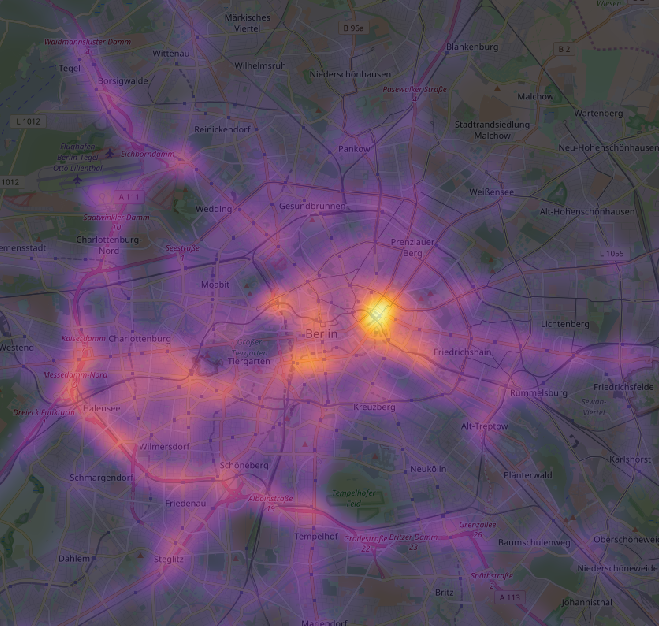
\includegraphics[width=0.9\textwidth]{images/points_berlin_heatmap.png}\\
	\caption{Heatmap of data point densities within the area of Berlin}
	\label{fig:introduction_ber_heat}
\end{figure}
\\
\autoref{fig:introduction_ber_heat} shows the heatmap of data points for Berlin area. We can see that most of the movements detected are on major train/tram/metro stations, highways and major living areas. 

\subsection{Data analysis}
\label{cha:introduction_dataanaly}

Statistics performed using tool written in Python (https://github.com/mrow4a/macroscopic-movements-algorithm-prototypes) shows, that for users at least once visiting Berlin, had in average 17 points gathered because of their movements in the period of 24h, harmonic mean of 4 points and maximum 100 of points.

\autoref{fig:introduction_ber_stats} shows that there is significant fraction of points which timestamp or distance did not change, thus duplicated point has been recorded. 
\\
TODO: This needs to be investigated
\\
\begin{figure}[!ht]
	\centering
	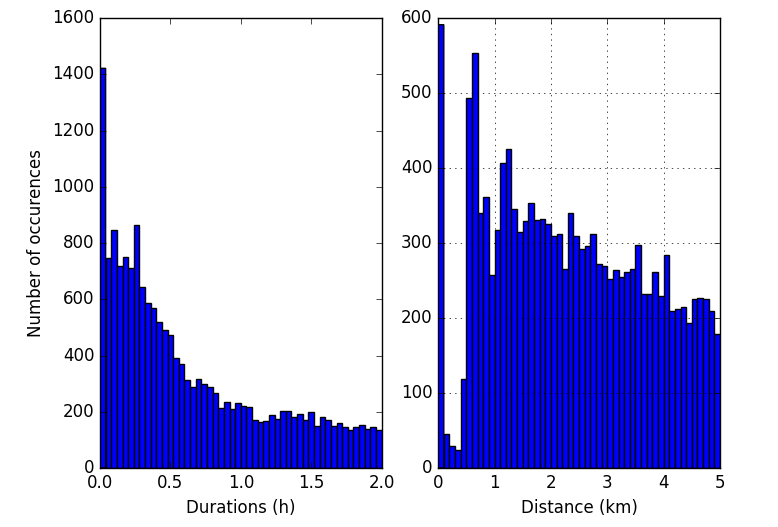
\includegraphics[width=0.6\textwidth]{images/berlin_stats_intro.png}\\
	\caption{Histograms of durations and distances between consecutive points under 5 km and under durations of 2h for the area of Berlin}
	\label{fig:introduction_ber_stats}
\end{figure}
\\\\
Furthermore, majority of durations between points is within interval of 30 minutes. For distances between points, there is significant "jump" at 500-1000m and 1100-1500m, which might mean that at these intervals, continuous points been gathered, and distances over that values might be discontinuous (ref. \autoref{fig:introduction_movement_update} ). It is due to the fact that these distance intervals are most frequent and that might suggest that this is an average "update" distance for the moving mobile devices, as described in \autoref{cha:introduction_methodo}. Less frequent values might suggest that updates were obtained with lower accuracy (e.g. by presence inside the building, metro line or simply mobile device lag in obtaining its location) and are result of discontinuity between consecutive updates.
\begin{figure}[!ht]
	\centering
	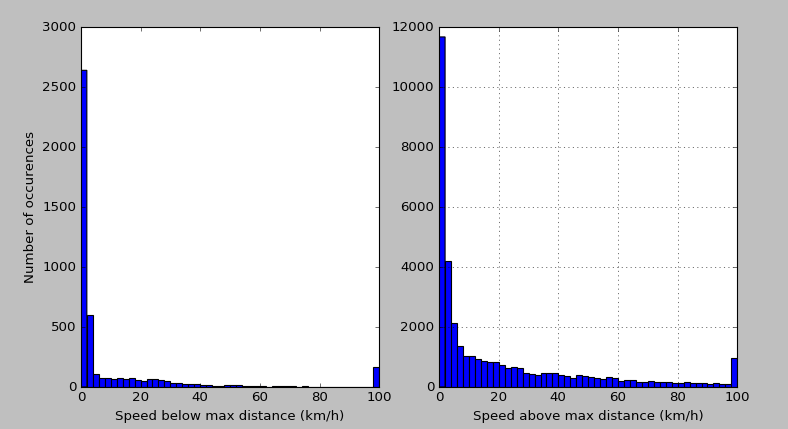
\includegraphics[width=0.6\textwidth]{images/berlin_speeds_distances.png}\\
	\caption{Histogram of speed between points with corresponding distance above or below 1.5 km}
	\label{fig:introduction_ber_sp_dis}
\end{figure}
\\
\autoref{fig:introduction_ber_sp_dis} shows that considering the registered distances within range of 1500m, the wast majority of points are between 0-2 km/h, and also significant interval at 2-6 km/h. The rest of the values is sparse distributed in interval 6-100+ km/h. In case of registered point above range of 1500m, we observe that indeed most frequent occurrence is at interval of 0-4 km/h, however most are sparse distributed above 4 km/h, with most points being in interval of 4-20 km/h. 
\FloatBarrier

\section{Approaches to stop detection for localization services}
\label{cha:introduction_appr_stopdet}

Here we should explain different approaches

\subsection{Stop Detection analyzing repetitive appearance at location}

\subsection{Stop Detection based on continuous localization}

\subsection{Stop Detection based on mobility index}
\label{cha:introduction_mob_index_sect}

In the paper \cite{MobilityIndexGIS}, movement of mobile devices between cells (handovers) is considered. To detect the periods of slow movements of stops at the specific location, parameter called Mobility Index is considered. 
\begin{figure}[!ht]
	\centering
	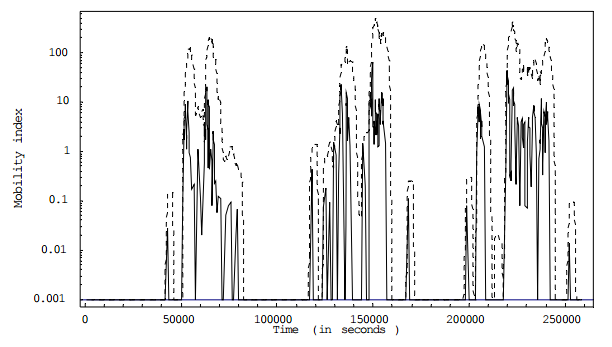
\includegraphics[width=0.5\textwidth]{images/intro_mobility_index.png}\\
	\caption{Mobility Index. Source: \cite{MobilityIndexGIS}}
	\label{fig:introduction_mob_index}
\end{figure}
\\
In a populated area, with many GSM cells, the mobile
terminal can change from one cell to another within
seconds or after several minutes. Given a set of consecutive records, the mobility of a user can be estimated by calculating the Mobility Index over a pre-defined time period (sliding window). The Mobility Index is the sum of the distance between each record and the previous ones, where the distance is the inverse of the time spent on each cell. If the value of MI is below certain threshold, it is assumed that the object stopped or moved slowly. 
\\\\
In the publication, sliding window of 10 minutes and a mobility index threshold value of 6 has been used for certain area. The obtained results were in agreement with actual movements during more than 90\% of the time. 
\\\\
High mobility index tells that user have been moving from checkpoint to checkpoint within very small time distance. Rapid drop in mobility index represents very long duration at the last point, and slight decrease in mobility index means that user changed position, but within longer duration.